\begin{figure}[H]
    \centering
    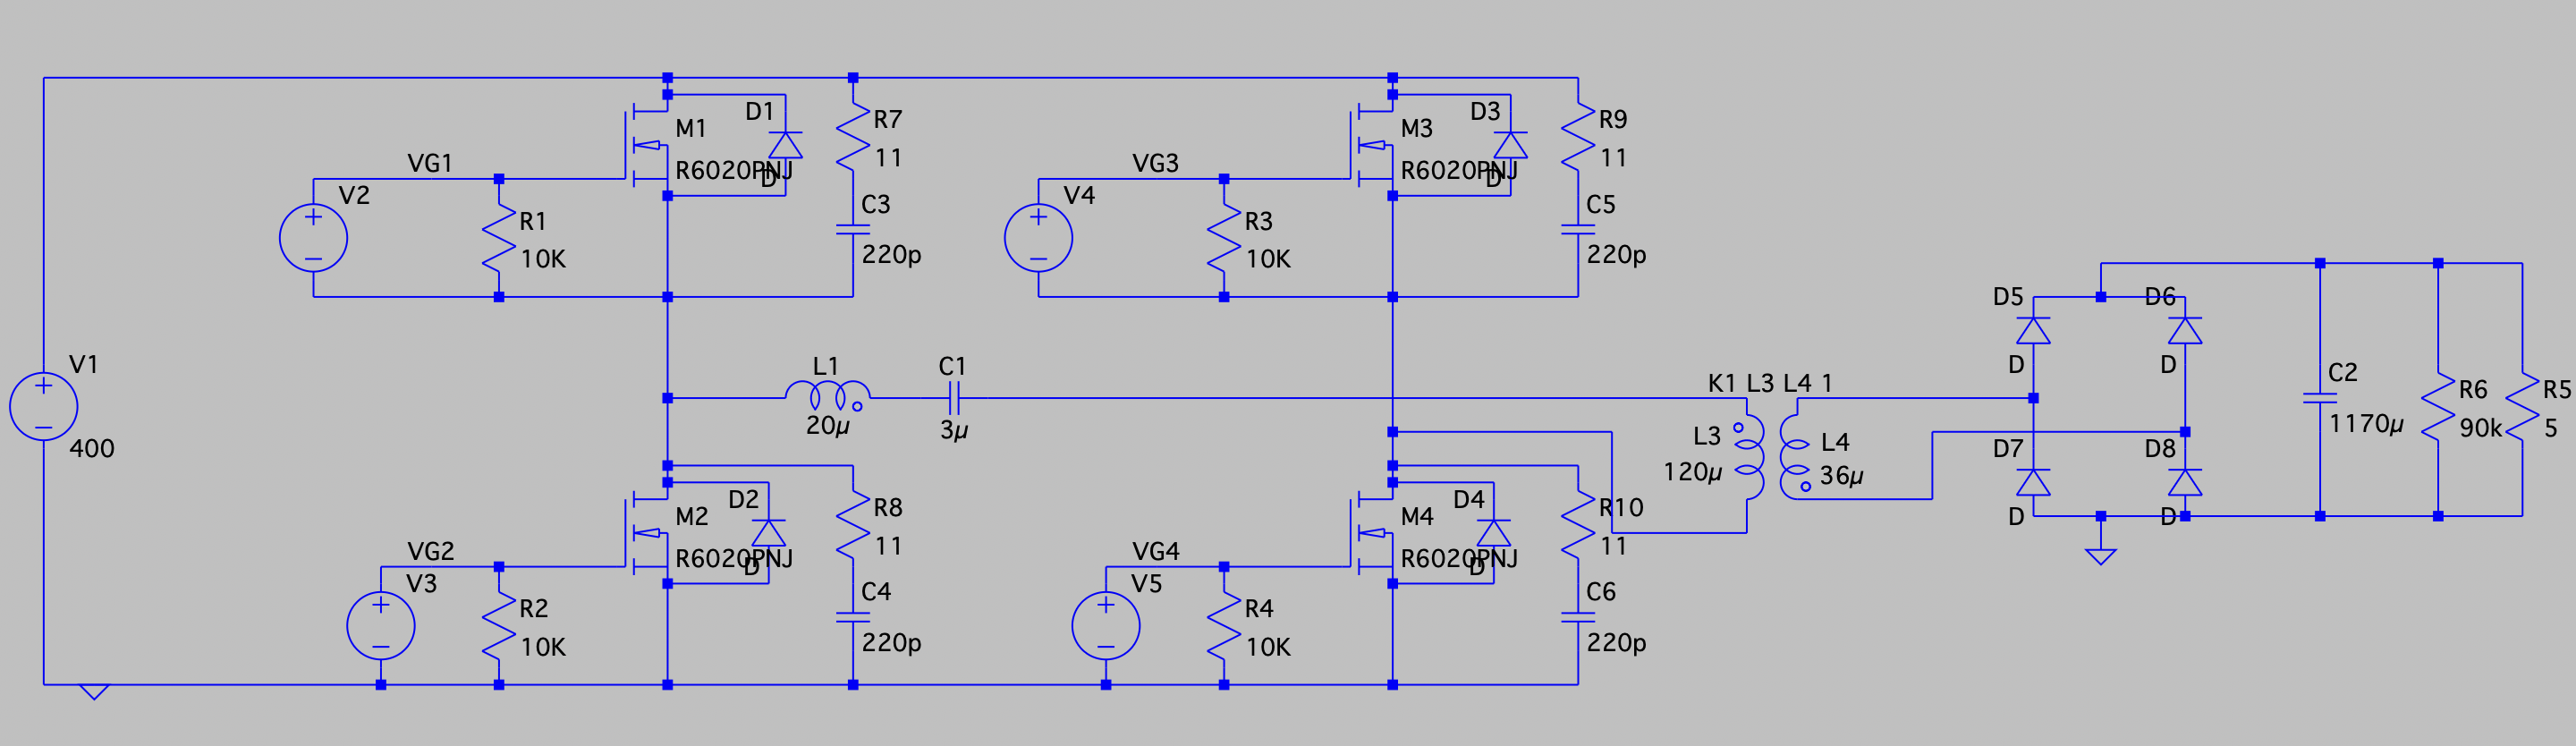
\includegraphics[width=\textwidth]{overall_circuit.png}
    \caption{Simulation}
    \label{fig:Simulation1}
\end{figure}

\subsection{Sectional Analysis}
One of my first tasks was to perform a sectional analysis of the complete motherboard and control board circuit.\\
\noindent
Since active feedback is not possible in LtSpice, I decided to split the complete circuit into multiple sections, such as gate driver circuit, switching circuit, voltage feedback op-amps and circuit, etc. and then simulate them individually.\\
\begin{figure}[H]
    \centering
    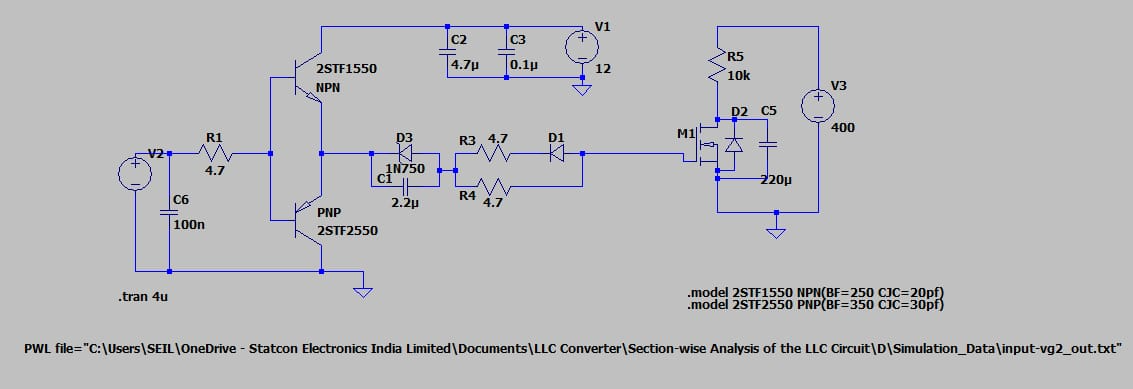
\includegraphics[width=\textwidth]{lt_circuit.png}
    \caption{Simulation}
    \label{fig:lt_circuit}
\end{figure}

\noindent
One such circuit is demonstrated in figure \ref*{fig:lt_circuit}

\subsection{Probing Actual Data}


\subsection{Comparitive Analysis of Simulated Data with Actual Data}
